\chapter{はじめに}
\thispagestyle{myheadings}


\section{背景}

位置を知るための技術は,人類の文明の発展とともに進化を続けてきた.
古代の航海士たちは太陽や北極星の観測により位置を測定し,
15世紀には六分儀の発明により天体の角度をより正確に測定できるようになった.20世紀に入ると,
電波技術の発展により地上の送信局からの電波を利用したロラン(LORAN: Long Range Navigation)が開発され,
これは後の衛星測位システムの基礎となる重要な概念を確立した.

% TODO 1.GPSについて語りすぎ感ある.削ってもよさそう
1973年にアメリカ国防総省によって開発が開始されたGPS(Global Positioning System)は,
位置測定技術に革命的な進歩をもたらした.
GPSは地球の周回軌道上に配置された複数の人工衛星からの電波を受信し,
地球上のどこでも高精度な位置測位を可能にした画期的なシステムである.
GPSは軌道高度約20,200kmの6つの軌道面に各4機ずつ,計24機以上の衛星を配置し,
地上管制局ネットワークにより衛星の軌道・時刻情報を管理している.

測位原理としては,衛星から送信される電波に含まれる軌道情報(エフェメリス)と原子時計による正確な時刻情報を利用する.
受信機は各衛星からの電波の伝搬時間を測定し,衛星までの距離(擬似距離)を算出する.
この擬似距離と衛星の位置情報を用いて,受信機の3次元位置(緯度,経度,高度)と時計誤差の4つの未知数を,
4機以上の衛星からの信号を同時に受信し幾何学的に解を得られる.

現代では,GPS以外にも複数の全球測位衛星システム(GNSS: Global Navigation Satellite System)が運用されている.
ロシアのGLONASS,EUのGalileo,中国のBeiDou,そして日本の準天頂衛星システム(QZSS)などが代表的である.
これらのシステムを組み合わせて,より高精度で信頼性の高い測位が可能となっている.
特に都市部では,複数のシステムを利用し,建物による衛星の遮蔽の影響を軽減できる利点がある.

しかし,GNSSには屋内環境での利用に大きな技術的制約が存在する.
GNSSの信号は高周波数帯(GPSの場合,L1帯:1575.42 MHz,L2帯:1227.60 MHz)を使用しているため,
建物の壁や天井などの建材を透過する際に著しく減衰する.
建材の種類や厚さ,信号の入射角などによって減衰量は異なるが,
一般的な建物内部では信号強度が受信機の検出限界を下回る状況が多く,測位そのものが困難となる.
また都市部においては建物による信号の遮蔽も深刻な問題となる.
高層ビルが密集する環境では,視認可能な衛星数が制限され,
測位に必要な4機以上の衛星からの信号を受信できない状況がある.
これらの要因により,屋内環境ではGNSSによる正確な位置測位が難しい問題がある.

一方で,屋内での位置測位へのニーズは年々高まっている.
人々が一日の大半を過ごす屋内空間において,
正確な位置情報は様々なサービスや業務の基盤となっている.
大規模商業施設では,買い物客への店舗情報の配信や経路案内により顧客満足度の向上が図られており\cite{burasapo},
来店客の動線分析から店舗レイアウトの最適化や混雑予測にも活用されている.
物流倉庫では,作業員と荷物の位置情報を組み合わせてより最適な経路案内や作業進捗管理が実現され,
人手不足が深刻化する業界において重要な解決策となっている.
特に近年では,IoTセンサーやスマートデバイスを活用した施設管理の高度化が加速している.
位置情報と連動した空調・照明の制御により,
人の滞在状況に応じた温度や明るさの自動調整が実現され,快適性を維持しながら消費エネルギーを最小化できる.
さらに,入退室管理システムと連携により,セキュリティの強化と利便性の向上も実現されている.

このような背景から,GNSSに依存しない屋内位置推定技術の研究開発が活発に行われている.
屋内位置推定手法は,空間内での絶対的な位置を求める手法(以下,絶対位置推定手法)と,
基準点からの相対的な位置を求める手法(以下,相対位置推定手法)に大別される.
空間内での絶対位置推定手法の代表的なものとして,電波を用いた測位手法がある.
これには主にWi-Fi測位とビーコン測位が含まれる.
これらの手法は,既知の位置に設置された送信機からの電波信号を利用して位置を特定する.
Wi-Fi測位では既存の無線LANインフラを活用できる利点があり,
ビーコン測位では電池駆動の小型送信機により柔軟な測位環境の構築が可能である.

電波を用いた測位手法には,主に3つのアプローチがある.
1つ目はProximity方式で,
もっとも強い電波を受信した送信機の位置を測位対象の位置とする単純な手法である.
2つ目はフィンガープリント(以下,FP)方式で,
事前に建物内の各地点で電波強度を測定してデータベース化し,
位置推定時には受信した電波強度パターンとデータベースを照合し位置を特定する.
3つ目はTriangulation方式で,3つ以上の送信機からの電波強度と既知の送信機位置情報を用いて,幾何学的に位置を算出する.
これらの手法の選択は,使用する技術や環境条件によって異なる.
Wi-Fi測位では複雑な屋内電波伝搬への対応からフィンガープリント方式が多く採用される一方,
ビーコン測位では設置の自由度を活かした近接法や三点測位が一般的である.

他の環境インフラを利用する手法として,地磁気測位がある.
この手法は,建物の鉄骨や設備機器により生じる地磁気の歪みパターンを位置推定に活用する.
地磁気の歪みパターンは建物内の位置によって異なる特徴を持つため,
これを位置推定の手がかりとして利用できる.
測位の際は,スマートフォンなどに搭載された地磁気センサーで測定した磁場ベクトルのパターンと,
事前に作成した地磁気マップを照合し位置を特定する.
追加のインフラ設置が不要という利点がある一方で,
環境の変化により磁場が変動する可能性があり,地磁気マップの定期的な更新が必要となる場合がある.

相対位置推定手法として,Dead Reckoning(自律航法)がある.Dead Reckoningは,
既知の出発点から移動体の速度と方位の時系列データを用いて,現在位置を推定する手法である.
この手法は古くから航海で用いられており,船舶の速度と進路から現在位置を推定していた.
現代では,自動車,ロボット,歩行者など,様々な移動体の位置推定に応用されている.

Dead Reckoningの1つとして,歩行者の位置推定に特化したPDR(Pedestrian Dead Reckoning:歩行者自律航法)がある.
PDRは歩行者の移動を逐次的に追跡し相対的な位置を推定する手法である.
% TODO 3. 何か文章がおかしい
この手法では,スマートフォンなどに搭載された慣性センサー(加速度センサー,ジャイロスコープ)を利用する.
PDRにおける位置推定は,歩行検出,歩幅推定,方位推定の3つの要素から構成される.

歩行検出では,加速度センサーの出力波形から歩行動作に特徴的な周期的なパターンを検出する.
人間の歩行動作では,着地時に特徴的な加速度変化が観測されるため,
この波形パターンの解析により歩行のタイミングを特定できる.

歩幅推定では,検出された各歩行動作における移動距離を推定する.
もっとも基本的な手法では,歩行者の身長から平均的な歩幅を設定する.
より高度な手法では,加速度波形の特徴量(ピーク値や周期など)から歩幅を動的に推定する.
例えば,歩行速度が速くなると加速度の振幅が大きくなる傾向があるのを利用し,
加速度波形の振幅と歩幅の関係をモデル化する方法がある.

方位推定では,ジャイロスコープを用いて歩行者の進行方向の変化を検出する.
ジャイロスコープは角速度を計測するセンサーで,この出力を時間積分し方位の変化量を算出できる.
ただし,ジャイロスコープの出力には常にわずかな誤差(バイアス誤差)が含まれており,
この誤差が積分過程で蓄積されていく.この問題への対策として,地磁気センサーやカメラなど,
他のセンサー情報を組み合わせて方位推定の精度を向上させる手法が研究されている.

PDRでは,これらの要素を組み合わせて歩行者の移動軌跡を推定する.
具体的には,歩行検出により得られた各ステップのタイミングにおいて,
推定された歩幅と方位の情報から,2次元平面上での移動ベクトルを計算する.
この移動ベクトルを初期位置から順次加算していくと,歩行者の移動軌跡が得られる.

相対位置推定手法と絶対位置推定手法には,それぞれ固有の課題がある.
絶対位置推定手法は特定の環境情報に依存するため,
その情報が得られない場所では位置推定の精度が低下する.
例えば,Wi-Fi測位では,アクセスポイントの設置位置が不明な場合や,
電波状況が不安定な場所では測位が困難となる.同様に,地磁気測位でも,
建物内の設備変更や金属物の移動により磁場環境が変化すると,
事前に作成した地磁気マップとの整合性が失われ,位置推定の精度が低下する.

一方,PDRによる相対位置推定では,初期位置と初期進行方向の情報が必須である.
これらの情報が不正確な場合,その後の推定結果全体に影響を及ぼす.
さらに,センサーの誤差が累積的に蓄積されるという本質的な課題がある.
例えば,ジャイロスコープによる方位推定では,センサーのわずかな誤差が時間とともに蓄積され,
推定される移動方向が実際の方向から徐々にずれていく.
また,歩幅推定においても,歩行者の歩容変化や床面の傾斜により誤差が生じ,
これも歩行距離とともに蓄積される.その結果,長時間の歩行では推定位置が実際の位置から大きく乖離してしまう.

これらの課題を解決するアプローチとして,PDRと環境情報を組み合わせたハイブリッド手法が注目されている.
PDRは連続的な位置推定が可能で,短時間であれば高い精度を維持できる一方,時間経過とともに誤差が蓄積する.
これに対し,Wi-Fi測位などの絶対位置推定は,環境情報が利用可能な場所では信頼性の高い位置情報を提供できる.
この2つの手法を適切に組み合わせによって,PDRの誤差蓄積を抑制しつつ,連続的な位置推定が可能となる.
例えば,Wi-Fi測位が可能な地点でPDRの累積誤差を補正したり,
地磁気の特徴的なパターンを検出した際に方位推定の精度を向上させたりする手法が提案されている.

さらに,実際の屋内環境では階層をまたぐ移動も一般的であり,3次元空間での位置推定の重要性が増している.
しかし,これまでの研究の多くは2次元平面上での位置推定に焦点を当てており,
階層判定を含む3次元空間での位置推定については十分な検討がなされていない.
また,これらのハイブリッド手法は環境条件や用途に応じて適切な組み合わせを選択する必要がある.
例えば,Wi-Fiインフラが充実している商業施設では,PDRとWi-Fi測位の組み合わせが効果的である一方,
建物の構造上,特徴的な地磁気分布が期待できる施設では,PDRと地磁気測位の組み合わせが有効となる.
利用可能な環境情報は建物によって大きく異なり,すべての環境で同じ手法を適用するのは困難である.


% TODO2. ここで入れるべきかわからないが軌跡を導出して補正するというアプローチ自体が新しい
% 一般的な位置推定は軌跡を出してそれを全体最適化というアプローチをとらないきがする
% その点が新しいかもしれない

\section{目的とアプローチ}

屋内位置推定システムの実用化が進む中,環境条件の多様性への対応と3次元空間での位置推定が重要な課題となっている.
位置推定システムの開発者は,各環境に適した手法を個別に実装する必要があり,
開発効率の低下や品質の不均一化といった問題が生じている.また,環境条件が変化した際の対応も困難である.

本研究の概要を図\ref{fig:overview}に示す.
本研究は,様々な環境条件や利用可能なセンサー情報に柔軟に対応可能な,PDRベースの3次元屋内位置推定アルゴリズムライブラリの開発を目的とする.
特に,複数階層を持つ建物内での継続的な位置推定を実現するため,水平方向の位置推定に加えて,
階層判定を含む垂直方向の移動推定も考慮する.
具体的には,以下の3つの要件を満たすライブラリの実現を目指す.

\begin{enumerate}
    \item PDRを基盤としつつ,利用可能な補助情報に応じて適切なアルゴリズムを組み合わせられる柔軟なフレームワークの提供
    \item 環境条件の変化と3次元空間での移動に対応可能な補正アルゴリズム群の実装
    \item 実装者が個々の利用環境に最適化された位置推定システムを容易に構築できる直感的なAPIの設計
\end{enumerate}

これらの目的を達成するために,本研究では以下のアプローチを採用する.

第一に,PDRを基盤技術として採用し,その基本機能を独立性の高いコンポーネントとして設計する.
PDRは追加のインフラ整備を必要としない特徴であり,3次元空間を含む様々な環境における位置推定の基盤として適している.
このPDRの基本機能をコンポーネント化し,環境条件や要求精度に応じた柔軟な機能選択を可能とする.

第二に,環境情報を活用した段階的な補正アプローチを導入する.
このアプローチでは,利用可能な環境情報に応じて適切な補正手法を選択・適用する.
例えば,フロアマップが利用可能な環境では物理的な移動制約を考慮した補正を行い,
気圧センサーのデータが利用可能な場合は階層判定による垂直方向の移動推定を行う.
この段階的な補正により,様々な環境条件に対応した3次元位置推定の実現を目指す.

第三に,拡張性と再利用性を重視したソフトウェアアーキテクチャを採用する.
これにより,新たな補正アルゴリズムの追加や,既存アルゴリズムの組み合わせを容易にし,
環境条件の変化への柔軟な対応を可能とする.
また,実装者が直感的に理解・使用できるインターフェースを提供し
個々の利用環境に最適化された位置推定システムの構築を支援する.

このように,本研究で提案するライブラリは,環境条件に応じて適切な手法を選択・組み合わせることで,
3次元空間における様々な状況に適応可能な屋内位置推定を実現する.
また新たなアルゴリズムやセンサー情報の追加にも柔軟に対応できる拡張性を備え,将来的な技術発展にも対応可能な基盤を提供する.

\begin{figure}[h]
	\centering
	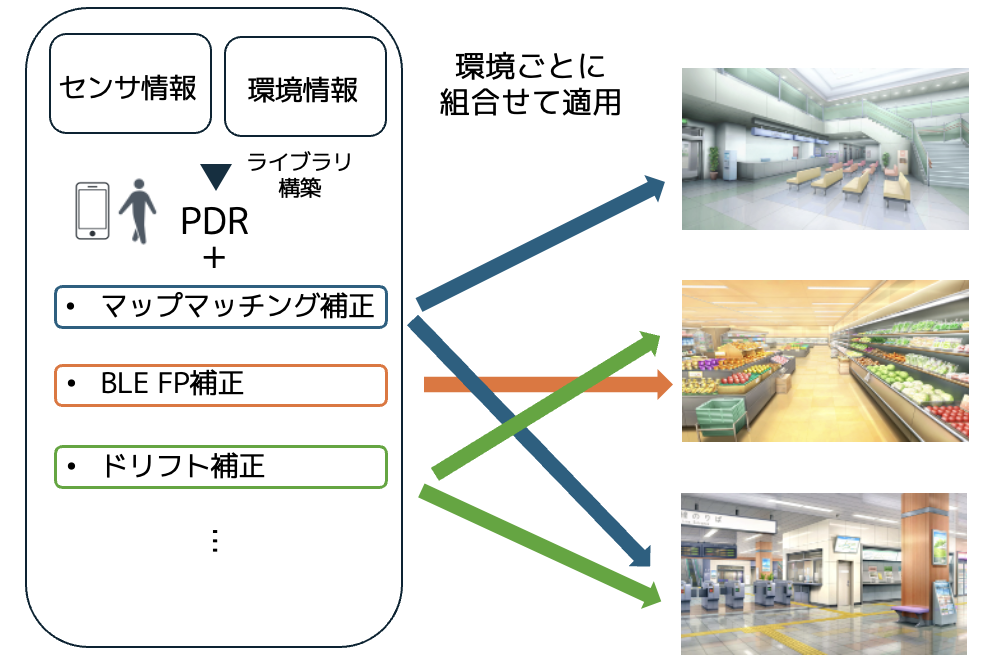
\includegraphics[width=\linewidth]{image/first.png}
	\caption{様々な環境や状況に対応できるPDRベースの\\3次元屋内位置推定ライブラリの概要}    \label{fig:overview}
\end{figure}

\section{論文構成}
本稿の構成は以下の通りである.2 章では,屋内位置推定に関する研究及びPDRライブラリに
関連する事例を提示し,本研究との関連性を述べる.
3 章では,ライブラリの要求仕様とライブラリの実装について述べる.
4 章では,ライブラリの検証と他環境における適用可能性の検討について述べる.
最後に5 章では,まとめと今後の課題について述べる.


